%%%%%%%%%%%%%%%%%%%%%%%%%%%%%%%%%%%%%%%%%%%%%%%%%%%%%%%%%%%%
%%% LIVECOMS ARTICLE TEMPLATE FOR BEST PRACTICES GUIDE
%%% ADAPTED FROM ELIFE ARTICLE TEMPLATE (8/10/2017)
%%%%%%%%%%%%%%%%%%%%%%%%%%%%%%%%%%%%%%%%%%%%%%%%%%%%%%%%%%%%
%%% PREAMBLE
\documentclass[9pt,bestpractices]{livecoms}
% Use the 'onehalfspacing' option for 1.5 line spacing
% Use the 'doublespacing' option for 2.0 line spacing
% Use the 'lineno' option for adding line numbers.
% The 'bestpractices' option for indicates that this is a best practices guide.
% Omit the bestpractices option to remove the marking as a LiveCoMS paper.
% Please note that these options may affect formatting.

\usepackage{lipsum} % Required to insert dummy text
\usepackage[version=4]{mhchem}
\usepackage{siunitx}
\usepackage{bm}
\DeclareSIUnit\Molar{M}
\usepackage[italic]{mathastext}
\newcommand{\versionnumber}{1.0}  % you should update the minor version number in preprints and major version number of submissions.
\newcommand{\githubrepository}{\url{https://github.com/dmzuckerman/Sampling-Uncertainty}}  %this should be the main github repository for this article
\graphicspath{{figures/}}
%%%%%%%%%%%%%%%%%%%%%%%%%%%%%%%%%%%%%%%%%%%%%%%%%%%%%%%%%%%%
%%% ARTICLE SETUP
%%%%%%%%%%%%%%%%%%%%%%%%%%%%%%%%%%%%%%%%%%%%%%%%%%%%%%%%%%%%
\title{Best Practices for Quantification of Uncertainty and Sampling Quality in Molecular Simulations [Article v\versionnumber]}

\author[1*\authfn{1}]{Alan Grossfield}
\author[2*\authfn{1}]{Paul N. Patrone}
\author[3*\authfn{1}]{Daniel R. Roe}
\author[4*\authfn{1}]{Andrew J. Schultz}
\author[5*\authfn{1}]{Daniel W. Siderius}
\author[6*\authfn{1}]{Daniel M. Zuckerman}
\affil[1]{University of Rochester Medical Center, Department of Biochemistry and Biophysics}
\affil[2]{Applied Computational and Mathematics Division, National Institute of Standards and Technology}
\affil[3]{Laboratory of Computational Biology, National Heart Lung and Blood Institute, National Institutes of Health}
\affil[4]{Department of Chemical and Biological Engineering, University at Buffalo, The State University of New York}
\affil[5]{Chemical Sciences Division, National Institute of Standards and Technology}
\affil[6]{Department of Biomedical Engineering, Oregon Health \& Science University}

\corr{alan_grossfield@urmc.rochester.edu}{AG}
\corr{paul.patrone@nist.gov}{PNP}
\corr{daniel.roe@nih.gov}{DRR}
\corr{ajs42@buffalo.edu}{AJS}
\corr{daniel.siderius@nist.gov}{DWS}
\corr{zuckermd@ohsu.edu}{DMZ}

\contrib[\authfn{1}]{These authors contributed equally to this work.}

\blurb{This LiveCoMS document is maintained online on GitHub at \githubrepository; to provide feedback, suggestions, or help improve it, please visit the GitHub repository and participate via the issue tracker.\\
\bigskip
Contribution of the National Institute of Standards and Technology, not subject to US copyright.
}

%% Common symbols
\newcommand{\stdev}[1]{s\left( #1 \right)}
\newcommand{\stdevmean}[1]{s\left( #1 \right)}
\newcommand{\expval}[1]{\langle #1 \rangle}
\newcommand{\mean}[1]{\bar{#1}}
\newcommand{\expvar}[1]{\sigma_{#1}^2}
\newcommand{\var}[1]{s^2\left( #1 \right)}

%\presentadd[\authfn{3}]{Department, Institute, Country}
%\presentadd[\authfn{4}]{Department, Institute, Country}

%%%%%%%%%%%%%%%%%%%%%%%%%%%%%%%%%%%%%%%%%%%%%%%%%%%%%%%%%%%%
%%% PUBLICATION INFORMATION
%%% Fill out these parameters when available
%%% These are used when the "pubversion" option is invoked
%%%%%%%%%%%%%%%%%%%%%%%%%%%%%%%%%%%%%%%%%%%%%%%%%%%%%%%%%%%%
\pubDOI{10.XXXX/YYYYYYY}
\pubvolume{<volume>}
\pubyear{<year>}
\articlenum{<number>}
\datereceived{Month, Day, Year}
\dateaccepted{Month, Day, Year}

%%%%%%%%%%%%%%%%%%%%%%%%%%%%%%%%%%%%%%%%%%%%%%%%%%%%%%%%%%%%
%%% ARTICLE START
%%%%%%%%%%%%%%%%%%%%%%%%%%%%%%%%%%%%%%%%%%%%%%%%%%%%%%%%%%%%

\begin{document}

\begin{frontmatter} %NOTE: to make the document single column, just take out the {frontmatter} sentinels
\maketitle

\begin{abstract}
The quantitative assessment of uncertainty and sampling quality is essential in molecular simulation.
Many systems of interest are highly complex, often at the edge of current computational capabilities.  Modelers must therefore analyze and communicate statistical uncertainties so that ``consumers'' of simulated data understand its significance and limitations.  This article covers key analyses appropriate for trajectory data generated by conventional simulation methods such as molecular dynamics and (single Markov chain) Monte Carlo.  It also provides guidance for analyzing some `enhanced' sampling approaches.  We do not discuss \emph{systematic} errors arising, e.g., from inaccuracy in the chosen model or force field.
\end{abstract}

\end{frontmatter}

\section{Introduction: Scope and definitions}
\label{sec:scope}
\subsection{Scope}

Simulating molecular systems that are interesting by today's standards is a challenging task.  In addition to the various system-specific issues that modelers must address, questions often arise concerning, e.g. the best way to adequately sample the desired phase-space or estimate uncertainties.  And while these latter questions are not unique to molecular modeling, their importance cannot be overstated: the usefulness of a simulated result ultimately hinges on being able to confidently and accurately report uncertainties.  

This article therefore aims to provide best-practices for reporting simulated observables, assessing confidence in simulations, and deriving uncertainty estimates (more colloquially, ``error bars'') based on a variety of statistical techniques developed (in part) for physics-based sampling methods (e.g.\ molecular dynamics and Monte Carlo) and their associated ``enhanced'' counterparts.  As a general rule, we advocate a tiered approach to 

PNP: I'm still working on this; had to put it down for an hour for a meeting (1-3-18)

%PNP note: originally we had the phrase, "Some problems and systems may be better studied with cruder techniques and analyses, which will not be covered here."  This seems like an attempt to limit the scope, but I don't know what the original author had in mind.  What types of analyses are we ruling out versus keeping in?


%simulation studies attempting to quantify observables and derive reliable estimates of uncertainty (e.g., error bars) based on `standard' canonical sampling methods (e.g., molecular dynamics and Monte Carlo) and associated `enhanced' sampling methods.
%Some problems and systems may be better studied with cruder techniques and analyses, which will not be covered here.
This article also will not cover issues of systematic error arising from inaccuracy in force field (underlying model) or even from the simulation setup.
Rather, we will take raw trajectory data at face value, assuming it is a valid outcome given the underlying model.
We emphatically will \emph{not} assume that a trajectory has been sufficiently `equilibrated' or 'converged'.

\subsection{Key Definitions}

In order to make the discussion that follows more precise, we define key terms used in subsequent sections.
We caution that while many of these concepts are familiar, our terminology follows the {\it International Vocabulary of Metrology} (VIM)\citep{JCGM:VIM2012}, a standard that sometimes differs from the conventional or common language of engineering statistics. 
For additional information about or clarification of the statistical meaning of terms in the VIM, we suggest that readers consult the {\it Guide to the expression of uncertainty in measurement} (GUM)\citep{JCGM:GUM2008}.
For clarity, we highlight differences between conventional terms and the VIM in the section following the glossary.
In cases of lexical ambiguity, we hold to the definition of terms as given in the VIM.

%The reader should be familiar with a set of basic statistical and simulation concepts.
%[and we should provide links/refs for each.]

%NOTE FOR DAN S.  In some places I comment on definitions using ``Remarks'' that immediately follow the definition.  Not sure how well this format jibes with the rest of the doc.  Anyways, feel free to merge these remarks into the definitions if you think appropriate.

%NOTE FOR PAUL P. I've restructed the document a bit, applying the "one sentence per line" rule, which makes diff'ing the document easier.

% Reply to Dan S.: One sentence rule works for me

\subsubsection{Glossary of Statistical Terms}
\begin{itemize}
%terms added by PNP and DWS

\item {\bf Random quantity}: A quantity whose numerical value is inherently unknowable or unpredictable.

\smallskip

\textbf{\textit{Remark:}}  Informally speaking, we assume that a random quantity can be described in terms of a mean (or expected) value and a dispersion.  The latter characterizes the extent to which a {\it realization} of the random quantity differs from the mean.  More formally, we assume that the probability of a random variable $X$ taking value $x$ is given by $P(x)dx$, where $P(x)$ is a probably density and $dx$ is an infinitesimal width about $x$.

\smallskip

\textbf{\textit{Remark:}} Virtually all simulation tools (even those using quasi-random number generators) are deterministic.  As such, the output of any given simulation is never truly random, since it is the composition of knowable and predictable calculations.  However, it is generally infeasible to reproduce simulated calculations by hand, so that these are {\it in practice} unknowable.  Moreover, the chaotic nature of typical simulated systems leads to a situation in which the frequency of a given system configuration is well described by probability densities of statistical mechanics.  See Ref.~\cite{Leimkuhler} for more discussion of this rather deep point.

\item {\bf True value:}  The value of a quantity that is consistent with its definition and is the objective of an idealized measurement or simulation.

\smallskip
\textbf{\textit{Remark:}} Often the adjective ``true'' is dropped when reference to the definition is clear by context. \citep{JCGM:GUM2008,JCGM:VIM2012}
%Not sure that the last phrase is entirely consistent with GUM, although I'm not sure this is necessarily a problem.  To a certain extent, we may need to tailor the language of GUM/VIM to the audience at hand.
\smallskip

\textbf{\textit{Remark:}} Generally speaking, we use the descriptor ``true value'' in reference to quantities such as the expected value and standard deviation of a simulation output (were we able to run infinitely many simulations).
As these quantities are inherently unknowable, we can only estimate their values and associated uncertainties.

\item {\bf Standard Uncertainty}: Uncertainty in a result (e.g.\ prediction of a true value) as expressed in terms of a standard deviation.
\smallskip 

\textbf{\textit{Remark:}} The definition of standard uncertainty does not specify how to calculate the standard deviation.
This choice ultimately rests with the modeler and should be dictated by the details of the uncertainty relevant to the problem at hand.  

\item {\bf Arithmetic mean}: An estimate of the (true) expectation value of a random quantity. The arithmetic mean is given by the formula
  %
  \begin{equation}
    \bar{q} = \dfrac{1}{n} \sum_{k=1}^{n} q_k \label{def:arith_mean}
  \end{equation}
  %
  where $q_j$ is an experimental or simulated realization of the random variable and $n$ is the number of samples. 
\smallskip 
%PNP Note: I added "or simulated" after "experimental" in the line above

\textbf{\textit{Remark:}} It is straightforward to show that the arithmetic mean is a random quantity whose expectation value is that same as that of the $q_j$, provided the latter have a common mean.

\item {\bf Experimental standard deviation}: An estimate of the (true) standard deviation of a random variable, given by the formula
  % 
  \begin{equation}
    s\left(q_k\right) = \sqrt{\dfrac{\sum_{j=1}^n\left(q_j - \bar{q}\right)^2}{n-1}} \label{def:exp_st_dev}
  \end{equation}
  %
  where $q_j$, $\bar{q}$, and $n$ are as defined previously. 
  
\item {\bf Experimental standard deviation of the mean}: An estimate of the standard deviation of the distribution of the arithmetic mean, given by the formula
  % 
  \begin{equation}
    s\left(\bar{q}\right) = \dfrac{s\left(q_k\right)}{\sqrt{n}}. \label{def:exp_st_dev_mean}
  \end{equation}
  %
  \smallskip
  
\textbf{\textit{Remark:}} The experimental standard deviation of the mean characterizes the dispersion of the arithmetic mean relative to its expectation.
See \hyperref[def:exp_st_dev]{example link to definition of the experimental standard deviation}.
  
\item {\bf Precision}: The amount of variability in an estimate (e.g., based on repeating a given simulation protocol multiple times).  %Better sampling in an individual simulation leads to higher precision.  
%I commented out the last phrase because ``better'' seems a bit vague to me in this context.  Should this comment be placed elsewhere?  
  
  
\item {\bf Accuracy}: The degree to which a result agrees with a reference value.
The latter may be an experimental measurement or the result of a well-sampled simulation.  
  
\item {\bf Raw data}: The numbers that the computer program directly generates as it proceeds through a sequence of states [the phase-space trajectory for molecular dynamics (MD) or the Markov chain for Monte Carlo (MC)].
For example, a MC simulation generates a sequence of configurations, for which there are associated properties such as the instantaneous pressure, temperature, volume, etc.
% NOTE FOR DAN S.  Programs also directly compute things like pressure, temperature, volume, etc., which are necessary for controlling thermostats, barostats, etc.  Should we include these in the list of raw data?
% DWS REPLY: How is this modification?
% PNP REPLY: Overall fine.  I changed Monte Carlo to MD in the last sentence.  Do MC simulations have associated pressures?  I always thought that could only be computed in the context of a dynamical simulation.
% DWS REPLY2: I switched it back to MC - one of my objectives in this paper to make sure it is not too MD-centric. Aside: yes, you can calculate an instantaneous pressure in MC via the molecular virial if using a fixed-N ensemble.
  
\item {\bf Derived observables}: Quantities derived from `non-trivial' (and often non-linear) analyses of raw data, e.g., properties that may not be computed for a single configuration such as free energies.
  
\item {\bf Indepent observables}: Random quantities $x$ and $y$ for which the joint probability density can be written as a product of individual probability densities $P(x,y)=P(x)P(y)$.  
  
\item {\bf (Linearly) Uncorrelated observables}:  If quantities $q_j$ and $q_k$ have mean values $\left< q_j \right> $ and $\left< q_k \right>$, then $q_j$ and $q_k$ are linearly uncorrelated if
% 
\begin{equation}
  \left< \left(q_j - \left<q_j\right> \right) \left(q_k - \left<q_k\right> \right) \right>=0
\end{equation}
%
where $\left< \star \right>$ denotes the (true) expectation value.

\smallskip

\textbf{\textit{Remark:}} Independence of random variables implies that they are linearly uncorrelated.  The converse, however, is not true.  

\smallskip

\textbf{\textit{Remark:}} In practice, it is easier to (empirically) show that random variables are uncorrelated than independent.  However, linear correlations are often all that are needed to arrive at uncertainty estimates for various quantities.  See, e.g.\ the discussion of correlation times and autocorrelation analyses.
%PNP: where is that discussion?



\item {\bf Correlated observables}: Random quantities that are not independent.

\item {\bf Correlation time}: In time-series data of a random quantity $q(t)$ (e.g.\ a physical property from a MC or MD trajectory), this is the time $\tau$ over which $q(t)$ and $q(t+\tau)$ remain (linearly) correlated.

\smallskip

\textbf{\textit{Remark:}} Generally speaking, MC and MD trajectories generate new configurations from preceding ones.
Thus, the correlation time can be interpreted as the time over which the system retains memory of its previous states.
Such correlations are often {\bf stationary}, meaning that $\tau$ is independent of $t$.
Roughly speaking, the total simulation time divided by the longest correlation time yields an estimate of the number of {\it uncorrelated} samples generated by a simulation.


%The time over which realizations of a random quantity indexed by a time-series (e.g.\ a physical property from a Monte Carlo or molecular dynamics trajectory) retain ``memory'' of one another, since each configuration is generated from the preceding one. Roughly, the total simulation time divided by the (longest) correlation time gives an estimate of the number of \emph{independent} samples that will govern overall statistical quality of the data.

\item {\bf Two-sided confidence interval}: A statistically derived bound pair of lower and upper bounds between which the (true) expectation value of a random quantity is likely to fall, as quantified by a {\it confidence level} (typically given as a percentage, e.g., 95~\%). The confidence level, in conjunction with the sample size, determines the {\it coverage factor}, which is multiplied by \hyperref[def:exp_st_dev_mean]{$s\left(\bar{q}\right)$} to assign the bounds of the confidence interval.

% Older versions
%\item Precision: The amount of variability in an estimate (based on repeating a given simulation protocol multiple times).
%      Better sampling in an individual simulation leads to higher precision.
%      The standard error of the mean is usually the key measure of the \emph{scale} of the statistical uncertainty - i.e., %precision.
%    \item Confidence Interval: A statistically derived pair of minimum and maximum values within which the mean of an observable is likely to fall, as quantified by a percentage.  Note that useful confidence intervals (e.g., 90 or 95\%) tend to be roughly \emph{four times} the standard error of the mean (from minimum to maximum).
%    \item Accuracy: The degree of agreement with a reference value, which may be an experimental measurement or the result of a %well-sampled simulation.
%    \item Raw data: The numbers that the computer program directly generates as it runs -- typically configurations, and also %velocities in molecular dynamics.
%    \item Derived observables:  Quantities derived from `non-trivial' analyses of raw data, such as free energies.
%    \item Correlation time: The time over which samples/configurations in a MC or MD trajectory retain some "memory" of one another, since each configuration is generated from the preceding one.  Roughly, the total simulation time divided by the (longest) correlation time gives an estimate of the number of \emph{independent} samples that will govern overall statistical quality of the data.

\end{itemize}

\subsubsection{Discussion of terminology}

As surveyed by Refs.~\citep{JCGM:GUM2008,JCGM:VIM2012}, the discussion that originally motivated many of theses definitions is rather philosophical.
Nonetheless, it bears repeating here, if only to force a level of honesty regarding what we can actually hope to achieve with simulations.

The fundamental idea underpinning this discussion is the observation that true values are inherently unknowable.
As an added twist, the {\it Uncertainty Approach} advocated by Ref.~\citep{JCGM:GUM2008} also points out that the {\it definitions of true values may be imprecise,} so that the latter are in fact not even uniquely defined.\footnote{The GUM treats this definitional uncertainty as negligible compared to other sources.
However, the notion of definitional uncertainty is worth revisiting in the context of simulated data.
For example, we are aware of at least one situation in which the large scale of noise in simulated data (as compared with experiments) induces subjectivity in the definition of the glass-transition temperature, which ultimately affects uncertainties in a non-trivial way.
See Ref.~\citep{patrone1} and \textcolor{red}{Cite TG doc}.}
As such, assignments of ``error'' are impossible to make, since these are defined relative to the true value.
Rather, statistical analyses are better interpreted as quantifying our state of knowledge, e.g., our ability to confidently state that the the ``true'' mean is within some interval.

From a practical standpoint, this leads one to revisit definitions of uncertainty as defined, for example, by Eqs.~\ref{def:exp_st_dev} and \ref{def:exp_st_dev_mean}.
Conventionally this has gone by the name ``standard error,'' but in keeping with the perspective already laid out, we advocate the use of \hyperref[def:exp_st_dev_mean]{experimental standard deviation of the mean}.
To maintain consistency with the VIM and GUM, we also use ``sample mean'' and ``sample standard deviation'' with their counterparts ``arithmetic mean'' and ``experimental standard deviation.''
The reader should be aware that this older language is still used frequently throughout the literature.


%Table of equivalencies

%Arithmetic mean = ``sample mean''\\
%Experimental standard deviation: ``sample standard deviation''\\
%Experimental standard deviation of the mean: ``standard error''\\


\section{Best Practices Checklist}

The self-contained checklist is presented on the following page.

\begin{Checklists*}[p!]
\begin{checklist}{Quantifying Uncertainty and Sampling Quality in Molecular Simulation}
\begin{itemize}
\item
  \textbf{Plan your study carefully by starting with pre-simulation sanity checks.}
  There is no guarantee that any method, enhanced or otherwise, can sample the system of interest.
  See Sec.\ \ref{sec:sanity}
    \begin{itemize}
    \item Consult best-practices papers on simulation background and planning/setup.
      See: \url{https://github.com/MobleyLab/basic_simulation_training}
    \item Estimate whether system timescales are known experimentally and feasible computationally based on published literature.
      If timescales are too long for straight-ahead MD, investigate enhanced-sampling methods for systems of similar complexity.
      The same concept applies to MC, based the number of MC trial moves instead of actual time.
    \item Read up on sampling assessment and uncertainty estimation, from this article or another source (e.g., Ref. \cite{Grossfield2009}).
      Understanding uncertainty will help in the \emph{planning} of a simulation (e.g., ensure collection of sufficient data).
      %- Key concept: Connection between the equilibrium ensemble and individual trajectory (may or may not reach equilibrium); equilibrium vs. non-equilibrium.
    \item Consider multiple runs instead of a single simulation.
      Diverse starting structures enable a check on sampling for equilibrium ensembles, which should not depend on the starting structure.
      Multiple runs may be especially useful in assessing uncertainty for enhanced sampling methods.
    %The starting structures should be as representative of the true ensemble as you can make them, and should be generated in an automated fashion (as opposed to using interactive setups) for better reproducibility,
    \item Check and validate your code/method via a simple benchmark system.
      See: \url{https://github.com/shirtsgroup/software-physical-validation}
    \end{itemize}
    \vspace{-0.325\baselineskip} %Line spacing after a sub-list is too large
    
\item
  \textbf{Do not ``cherry-pick'' data that provides hoped-for outcomes.}
  This practice is ethically questionable and, at a minimum, can significantly bias your conclusions.
  Use all of the available data unless there is an objective and compelling reason not to, e.g.\ the simulation setup was incorrect or a sampling metric indicated that the simulation was not equilibrated.
  When used, sampling metrics should be applied uniformly to \emph{all} simulations to further avoid bias.
    
\item
\textbf{Perform simple, semi-quantitative checks which can rule out (but not ensure) sufficient sampling.} It is easier to diagnose insufficient sampling than to demonstrate good sampling.  See Sec.\ \ref{sec:quick}.
    \begin{itemize}
    \item Critically examine the time series of a number of observables, both those of interest \emph{and others}.
      Is each time series fluctuating about an average value or drifting overall?
      What states are expected and what are seen?
      Are there a significant number of transitions between states?
    %\item Plot as many properties as you can think of, even if they’re not interesting
    \item If multiple runs have been performed, compare results (e.g., time series, distributions, etc.) from different simulations.
    \item An individual trajectory can be divided into two parts and analyzed as if two simulations had been run.
    %\item If applicable, perform pairwise RMSD visual analysis for individual runs as described in Sec.\ \ref{sec:bio_RMSD}.
    %\item Plot pairwise configurational distances (e.g., RMSD values for biomolecules) in greyscale for $\sim$100 evenly spaced frames
    %\item Visualize the trajectory graphically -- look for slow motions.  BE SKEPTICAL!
    %\item Compare observable different fractions of a run (DMZ thirds idea)
    %\item Andrew: short vs. very short [DMZ: this would need to be described somewhere]
    %\item Daniel R: Compare runs from different initial conditions - be sure initial conditions are ‘different enough’
    \end{itemize}
        \vspace{-0.325\baselineskip} %Line spacing after a sub-list is too large

\item
  \textbf{Remove an ``equilibration'' (a.k.a. ``burn in'', or transient) portion of a single MD or MC trajectory} and perform analyses only on the remaining ``production'' portion of trajectory.  An initial configuration is unlikely to be representative of the desired ensemble and the system must be allowed to relax so that low probability states are not overrepresented in collected data.  See Sec.\ \ref{sec:equil}.
 
\item
  \textbf{Consider computing a quantitative measure of global sampling}, i.e., attempt to estimate the number of statistically independent samples in a trajectory.  Sequential configurations are highly correlated because one configuration is generated from the preceding one, and estimating the degree of correlation is essential to understanding overall simulation quality.
  See Secs.\ \ref{sec:global} and \ref{sec:autocorrelation}.

\item
  \textbf{Quantify uncertainty in specific observables of interest using confidence intervals.}
  The statistical uncertainty in, e.g.\ the \hyperref[def:arith_mean]{\emph{arithmetic mean}} of an observable decreases as more independent samples are obtained and can be much smaller than the \hyperref[def:exp_st_dev]{experimental standard deviation} of that observable.
  See Sec.\ \ref{sec:specific}.
 
\item
  \textbf{Use special care when designing uncertainty analyses for simulations with enhanced sampling methods.}
  The use of multiple, potentially correlated trajectories within a single enhanced-sampling simulation can invalidate the assumptions underpinning traditional analyses of uncertainty.
  See Sec.\ \ref{sec:enhanced}.

\item
\textbf{Report a complete description of your uncertainty quantification procedure, detailed enough to permit reproduction of reported findings.}
Describe the meaning and basis of uncertainties given in figures or tables in the captions for those items, e.g., "Error bars represent 95\% confidence intervals based on bootstrapping results from the independent simulations."
Provide expanded discussion of or references for the uncertainty analysis if the method is non-trivial.
Consider publishing unprocessed simulation data (measurements/observations) and post-processing scripts, perhaps using public data or software repositories, so that readers can exactly reproduce the processed results and uncertainty estimates. 
The non-uniformity of uncertainty quantification procedures in the modern literature underscores the value of clarity and transparency going forward.

\end{itemize}
\end{checklist}
\end{Checklists*}

\section{Pre-simulation sanity checks and planning tips}
\label{sec:sanity}

Sampling a molecular system that is complex enough to be ``interesting'' in modern science is likely to be extremely challenging.
Therefore, a small amount of effort spent planning a study can pay off many, many times over: in the worst case, weeks or months of simulation time followed by additional weeks or months of analysis can lead to insignificant conclusions in a poorly planned study.

If you read this guide through \emph{before} performing a simulation, you will have a much better sense of the criteria applicable to your data -- and which indeed \emph{should} be applied by knowledgeable reviewers of your work.
Thus we strongly advise understanding the concepts presented here as well as in related reviews \cite{Grossfield2009,JCGM:GUM2008}.

In a generic sense, the overall goal is to be able to draw statistically significant conclusions regarding a particular phenomenon or question of interest.
And ``good statistics'' follow from repeated observations of a phenomenon, which can only happen if the simulation length \emph{exceeds} the pertinent timescales.
One generic strategy that will allow you to at least understand your data in a self-consistent way is to perform several repeats of the same simulation protocol: as described below, repeats can be used to assess variance in \emph{any} observable, within the time you have run your simulation.
Also, it is essential to realize that a system may possess states (regions of configuration space) that, although important, are \emph{never} visited in a given simulation set because of insufficient computational time \cite{Grossfield2009}.

What are the pertinent timescales?
That's a question which has to be answered individually for each system.
You will want to study the experimental and computational literature for your particular system, although we warn that a published prior simulation of a given length does not in itself validate a new simulation of a similar or slightly increased length.
In the end, your data must be validated by statistical analyses, such as those described below.

[ADD DOUBLE-WELL FIGURE - caption to note dominant barrier may not be present]

A toy model can generically illustrate timescales and their effects on sampling.
Consider the double-well free energy landscape shown in Fig.\ XXXX, noting the slowest timescale is for crossing the largest barrier.
Generally, you should expect that the value of \emph{any} observable (e.g., $x$ itself or another coordinate not shown or a function of those coordinates) will depend on which of the two dominant basins the system occupies; and, in turn, the equilibrium average of an observable will require sampling the two basins according to their equilibrium populations.
In order to directly sample the equilibrium populations of the two basins, a trajectory will have to be many times the slowest timescale.
The relative populations of states are inferred from time spent in each state, which only will be representative if there are many transitions;
put another way, the equilibrium populations follow from the transition rates \cite{Zuckerman2011} which can be estimated from mulitple events.
For completeness, we note that there is no guarantee that sampling of a given system will be limited by a dominant barrier.  
Instead, a system could exhibit a generally rough landscape with many pathways between states of interest.
Nevertheless, the same cautions apply.

What should be done if a determination is made that a system's timescales are too long for direct simulation?
The two main options would be to consider a more simplified (``coarse-grained'') model or an enhanced sampling technique, bearing in mind that enhanced sampling methods are not foolproof but have their own limitations which should be considered carefully.

Lastly, whatever simulation protocol you pursue, be sure to use a well-validated piece of software.
If you are using your own code, check it against independent simulations on other software for a system that can be readily sampled.
[benchmark systems???]


% !TEX root = ./main.tex

\section{Quick-and-Dirty checks that can rule out good sampling}
\label{sec:quick}

It is difficult to establish with certainty that good sampling has been achieved, but it is not difficult to \emph{rule out} high-quality sampling.
Here we elaborate on some quick-and-dirty tests that quickly show inadequacies in sampling.

\subsection{Zeroth-order system-wide tests}

The simplest test for poor sampling is lack of equilibration: if the system is still noticeably relaxing from its starting conformation, statistical sampling has not even begun, and thus by definition is poor.  As a result, the very first test should be to verify that the basic equilibration has occurred.  To check for this, one should inspect the time series for a number of simple scalar values, such as potential energy, system size (and area, if you are simulating a membrane or other system where one dimension is distinct from the others), temperature (if you are simulating in the NVE ensemble), and/or density (if simulating in the isothermal-isobaric ensemble).  Often, simple visual inspection is sufficient to determine that the simulation is systematically changing, although more sophisticated methods have been proposed by Chodera \cite{Chodera-2016}.  If \emph{any} value appears to be systematically changing, then the system is not equilibrated.

\subsection{Tests based on configurational distance measures - e.g., RMSD for biomolecules}

\begin{wrapfigure}{r}{6cm}
  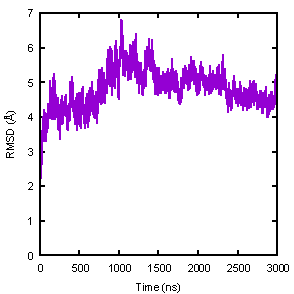
\includegraphics[width=5.8cm]{figures/rmsd/rmsd}
  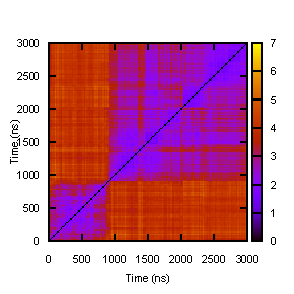
\includegraphics[width=5.8cm]{figures/rmsd/rmsds}
  \caption{
  \label{f:rmsd} RMSD as a measure of convergence.  The upper panel shows the
  $\alpha$-carbon RMSD of the protein rhodopsin from its starting structure as a
  function of time.  The lower panel shows the all-to-all RMSD map computed from the same
  trajectory.  Data from Leioatts, et al \cite{Grossfield-2015}.
  }
\end{wrapfigure}

We will use the standard biomolecular RMSD (root mean-squared difference) as a generic distance measure for illustrative purposes.
Alternatives to RMSD could be a dihedral-angle distance or another measure specific to your system of interest.
Note that RMSD, like any distance in a high-dimensional space, becomes ``degenerate'' for larger values: given a reference configuration, there are a large number of configurations which differ from the reference by a given large RMSD. This is analogous to the increasing number of points in three-dimensional space with increasing radial distance from a reference point, except much worse because of the dimensionality. For a detailed exploration of expected RMSD distributions for biomolecular systems see the work of Pitera.\citep{Pitera2014}

Some qualitative tools for assessing global sampling based on RMSD were reviewed
in prior work \cite{Grossfield2009}.   The classic time series plot of RMSD with
respect to a crystal or other single reference structure can immediately
indicate whether the structure is still systematically changing.  Although this
kind of plot was historically used as a sampling test, it should really be
considered as another equilibration test like those discussed above.  Moreover,
it's not even a particularly good test of equilibration, because the degeneracy
of RMSD means you can't tell if the simulation is exploring new states that are
equidistant from the chosen reference.  The upper panel of Figure \ref{f:rmsd}
shows a typical curve of this sort, taken from a simulation of the G
protein-coupled receptor rhodopsin \cite{Grossfield-2015}; the curve increases
rapidly over the few nanoseconds and then roughly plateaus.  It is difficult to
assign meaning to the other features on the curve.

A better RMSD-based convergence measure is the all-to-all RMSD plot; taking the
RMSD of each snapshot in the trajectory with respect to all others allows you to
use RMSD for what it does best, identifying very similar structures.  The lower
panel of Figure \ref{f:rmsd} shows an example of this kind of plot, applied to
the same trajectory before.  By definition, all such plots have values of zero
along the diagonal, and occupation of a given state shows up as a block of
similar RMSD along the diagonal; in this case, there are 2 main states, with one
transition occuring roughly 800 ns into the trajectory.  Off diagonal ``peaks''
(regions of low RMSD between structures sampled far apart in time) indicate that
the system is revisiting previously sampled states, a necessary condition for
good statistics.  In this case, the initial state is never sampled after the
first transition, but there are a number of small transitions within the second
state.

\subsection{Assessing Convergence}
Convergence in the context of biomolecular simulations typically refers to the overlap of two independent measurements of the same property. If a measure is not converged it is a strong indication that sampling is poor. There are two common ways to try to obtain independent measurements. Arguably the best way is to have multiple independent simulations, each with varying initial starting conditions. Ideally these starting conditions should in some way span the space to be sampled; this way one can have confidence that simulations are not being trapped in a local minimum. For example, say the goal is to sample the phi and psi torsions of alanine dipeptide: the phi and psi angles for one simulation could be started from an alpha-helical conformation, while another simulation could be started from a polyproline II conformation. It is important to note that the starting conditions only need to be varied enough so that the desired space is sampled. For example, if the goal is to sample protein folding and unfolding, there should be some simulations started from the folded conformation and some from the unfolded, but if it is not important to consider protein folding no initial conformation needs to be unfolded.

Another way to obtain independent measurements is to divide a single simulation into two or more subsets. However this can at times be problematic because it can be more difficult to tell if the system is trapped in a local minimum since there is a single starting point. Those employing this approach should take extra care to assess their results (see in particular sections on 'block averaging' below).

There are two simple ways to compare independent measurements of a property. The simplest is to compare the arithmetic means and standard deviations. If these values do not overlap then convergence has not been achieved. However, since this assumes that the values are normally distributed, a better way is compare the overlap of the probability distributions (i.e. the histograms). This can be done via Kullback-Leibler or Jensen-Shannon divergence.
% !TEX root = ./main.tex

\section{Determining and removing an equilibration or `burn-in' portion of a trajectory}
\label{sec:equil}

\begin{figure}
  \centering
  % 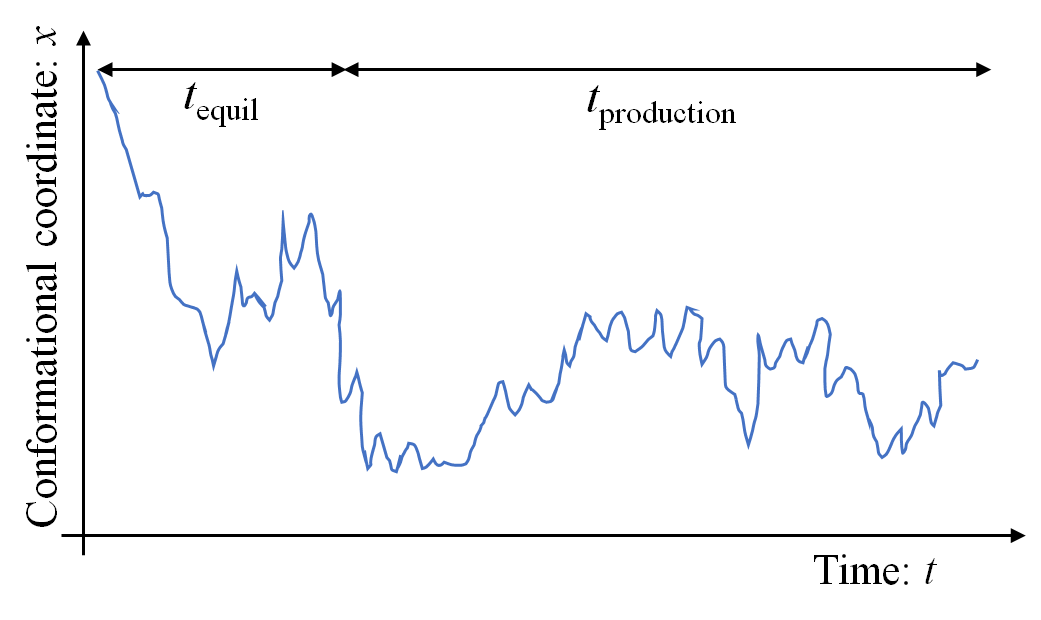
\includegraphics[width=7cm]{figures/tequil-time-trace}
  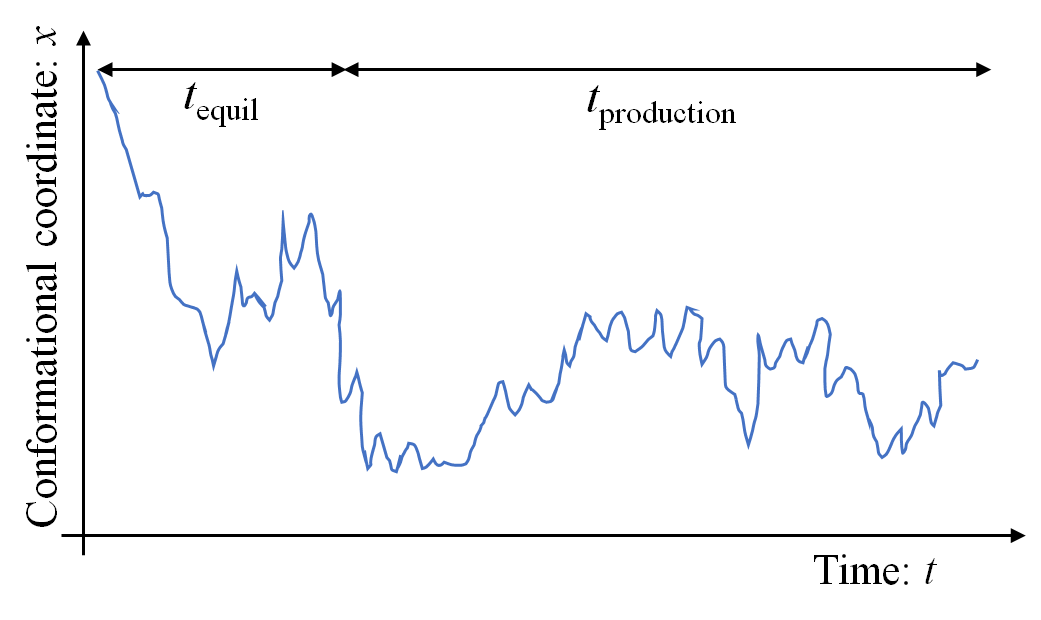
\includegraphics[width=0.9\linewidth]{figures/tequil-time-trace}
  \caption{
  \label{fig:tequil}
  The equilibration and production segments of a trajectory.
  ``Equilibration'' over the time $t_{\mathrm{equil}}$ represents transient behavior while the initial configuration relaxes toward configurations more representative of the equilibrium ensemble.
  Readers are encouraged to select $t_{\mathrm{equil}}$ in a systematic way based on published literature.
  If you find strong sensitivity of ``production'' data to the choice of $t_{\mathrm{equil}}$, this suggests additional sampling is required.
  }
\end{figure}

The ``equilibration'' or ``burn-in'' time $t_{\mathrm{equil}}$ represents the initial part of a single continuous trajectory (whether from MD or MC) that is \emph{discarded} for purposes of data analysis of \emph{equilibrium or steady-state properties};
the remaining trajectory data are often called ``production'' data.
See Fig.\ \ref{fig:tequil}.
Discarding data may seem counter-productive, but there is no reason to expect that the initial configurations of a trajectory will be important in the ensemble ultimately obtained.
Including early-time data, therefore, can systematically \emph{bias} results.

To illustrate these points, consider the process of relaxing an initial, crystalline configuration of a protein to its amorphous counterpart in an aqueous environment.
While the initial structure might seem to be intrinsically valuable, remember that configurations representative of the crystal structure may never appear in an aqueous system.
As a result, the initial structure may be subject to unphysical forces and/or transitions that provide useless, if not misleading information about the system behavior.\footnote{In MD modeling of structural polymers (e.g., thermoset polymers), the problem of unphysical forces can be so severe that simulations become numerically unstable and crash.  This frequently manifests as systems that explode and/or tear themselves apart.  As a result, relaxation is often performed using Monte Carlo moves that minimize energy without reference to velocities and forces.}
Relaxation should therefore be viewed as a means to an end: we only care that the relaxed state is representative of {\it any} local energy-minimum that the system might sample, not how we arrived at that state.

The RMSD trace in Fig. \ref{f:rmsd} illustrates typical behavior of a system undergoing relaxation.  Note the very rapid RMSD increase in the first $\approx$ 200 ns. Part of this increase is simply entropic: the volume of phase space within 1 {\AA} of a protein structure is extremely small, so that the process of thermalizing rapidly increases the RMSD from the starting structure, \emph{regardless of how favorable or representative that structure is}.  Thus, examining that initial rapid increase is not helpful in determining an equilibration time.  However, in this case, the RMSD continues to increase past 3 {\AA}, which is larger than the amplitude of simple thermal fluctuations (shown by Fig.\ \ref{f:rmsd}B), indicating an initial drift to a new structure, followed by sampling.

Accepting that some data should be discarded, it is not hard to see that we want to avoid discarding too much data, given that many systems of interest are extremely expensive to simulate.  In statistical terms, we want to remove bias but also minimize uncertainty (variance) through adequate sampling.  Before addressing this problem, however, we emphasize that the very notion of separating a trajectory into equilibration and production segments only makes sense if the system has indeed reached configurations important in the equilibrium ensemble. While it is generally impossible to guarantee this has occurred, some easy checks for determining that this has not occurred are described in Sec.\ \ref{sec:quick}. \emph{It is essential to perform those basic checks before analyzing data with a more sophisticated approach} that may assume a trajectory has a substantial amount of true equilibrium sampling.

%\textcolor{red}{PNP comment: The below paragraph has a few ambiguities. See .tex file for my comments}
%\textcolor{green}{DMZ comment: I made some edits but it's not really my expertise.  I will ask John Chodera to clean it up for us.}
%PNP comment:  The sentence, "The key idea is to analyze data as a function of the amount of data removed," sounds oxymoronic.  Is the idea to track estimators of an observable as data in the corresponding time series is removed?  If so, consider rephrasing.  Also, how is bias monitored if we don't know the true value of the observable?  This needs to be flushed out a little more.  Also, how can the effective sample size increase as I remove data...?  I suspect that the burn-in time shifts the mean if I keep all of the data, so I have the appearance of small but long-time correlations.  If this intuition is correct, we should probably be a little more explicit.

A robust approach to determining the equilibration time is discussed in \cite{Chodera-2016}, which generalizes the notion of reverse cumulative averaging~\cite{Yang2004} to observables that do not necessarily have Gaussian distributions.
The key idea is to analyze time-series data considering the effect of discarding various trial values of the initial equilibration interval, $t_{\mathrm{equil}}$ (Fig.\ \ref{fig:tequil}), and selecting the value that maximizes the effective number of uncorrelated samples of the remaining production region.
This effective sample size is estimated from the number of samples in the production region divided by the number of temporally correlated samples required to produce one effectively uncorrelated sample, based on an auto-correlation analysis.
At sufficiently large $t_{\mathrm{equil}}$, the majority of the initial relaxation transient is excluded, and the method selects the largest production region for which correlation times remain short to maximize the number of uncorrelated samples.
Care must be taken in the case that the simulation is insufficiently long to sample many transitions among kinetically metastable states, however, or else this approach can simply result in restricting the production region to the last sampled metastable basin.
%As described by Chodera \cite{Chodera-2016}, one can monitor both the variance and the effective sample size, which is roughly quantified by the total simulation time considered divided by the auto-correlation time.
%If the transient data in the interval $t_{\mathrm{equil}}$ is anomalous and removed, one expects the variance to decrease.
%Chodera indicates that the effective sample size peaks at the optimal $t_{\mathrm{equil}}$, making the latter easy to discern.
%We caution that estimating the correlation time may require care, and 
Readers may want to compare auto-correlation times for individual observables to the global ``decorrelation time'' \cite{Lyman2007a} described in Sec.\ \ref{sec:global}.  
As another general check, if values of observables estimated from the production phase depend sensitively on the choice of $t_{\mathrm{equil}}$, it is likely that further sampling is required.



\section{Quantification of Global Sampling}
\label{sec:global}


With ideal trajectory data, one would hope to be able to compute arbitrary observables with reasonably small error bars.
During a simulation, it is not uncommon to monitor specific observables of interest, but after the data are obtained, it may prove necessary to compute observables not previously considered.
These points motivate the task of estimating global sampling quality, which can be framed most simply in the context of single-trajectory data:
``Among the very large number of simulation frames (snapshots), how many are statistically independent?''
This number is called the \emph{effective sample size.}
From a dynamical perspective evoking auto-correlation ideas, which also apply to Monte Carlo data, how long must one wait before the system completely loses memory of its prior configuration?
The methods noted in this section build on ideas already presented in Sec.\ \ref{sec:quick} on qualitative sampling analysis, but attempt to go a step further to quantify sampling quality.

We emphasize that \emph{no single method described here has emerged as a clear best practice.}
However, because the global assessment methods provide a powerful window into overall sampling quality, which could easily be masked in the analysis of single observables (Sec.\ \ref{sec:specific}), we strongly encourage their use.
The reader is encouraged to try one or more of the approaches in order to understand the limitations of their data.


A key caveat is needed before proceeding.
Analysis of trajectory data generally cannot make inferences about parts of configuration space not visited \cite{Grossfield2009}.
It is generally impossible to know whether configurational states absent from a trajectory are appropriately absent because they are highly improbable (extremely high energy) or because the simulation simply failed to visit them because of a high barrier or random chance.

\subsection{Global sampling assessment for a single trajectory}
Two methods applicable for a single trajectory were previously introduced by some of the present authors, exploiting the fact that trajectories typically are correlated in time.
That is, each configuration evolves from and is most similar to the immediately preceding configuration;
this picture holds for standard MD and Markov-chain MC.
Both analysis methods are implemented as part of the software package LOOS \cite{LOOS,LOOS-JCC}.

\begin{figure}
  \centering
  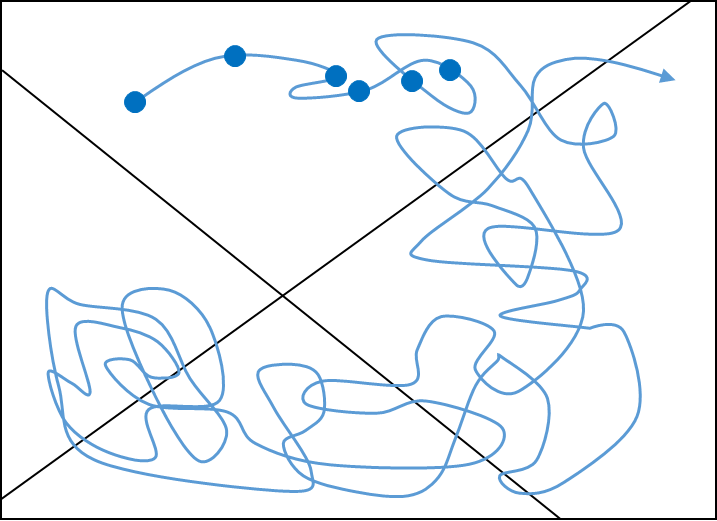
\includegraphics[width=0.8\linewidth]{decorr-graphic.png}
  \caption{The basis for ``decorrelation analysis'' \cite{Lyman2007a}.
  From a continuous trajectory (blue curve), configurations can be extracted at equally spaced time points (filled circles) with each such configuration categorized as belonging to one of a set of arbitrary states (delineated by straight black lines).  
  If the configurations are statistically independent -- if they are sufficiently decorrelated -- then their statistical behavior will match that predicted by a multinomial distribution consistent with the trajectory's fractional populations in each state.
  A range of time-spacings can be analyzed to determined if and when such independence occurs.}
  \label{fig:decorr}
\end{figure}

Lyman and Zuckerman proposed a global ``decorrelation'' analysis by mapping a trajectory to a discretization of configuration space (set of all $x, y, z$ coordinates) and analyzing the resulting statistics \cite{Lyman2007a}.
Configuration space is discretized into bins based on Voronoi cells of structurally similar configurations,  e.g., using RMSD defined in Eq.\ \ref{eq:rmsd} or another configurational similarity measure; reference configurations for the Voronoi binning are chosen at random or more systematically as described in \cite{Lyman2007a}.
Once configuration space is discretized, the trajectory frames can be classified accordingly, leading to a discrete (i.e., 'multinomial') distribution (Fig.\ \ref{fig:decorr}).
The analysis method is based on the observation that the variance for any bin of a multinomial distribution is known, given the bin populations (from trajectory counts) and a specified number of independent samples drawn from the distribution \cite{Lyman2007a}.
The knowledge of the expected variance allows testing of increasing waiting times between configurations drawn from the trajectory to determine when and if the variance approaches that expected for independent samples.
The minimum waiting time yielding agreement with ideal (i.e., uncorrelated) statistics yields an estimate for the decorrelation/memory time, which in turns implies an overall effective sample size. 



A second method, employing block covariance analysis (BCOM), was presented by Romo and Grossfield \cite{Romo2011} building on ideas by Hess \cite{Hess2002}.  In essence, the method combines two standard error analysis techniques --- block averaging \cite{Flyvbjerg-1989} and bootstrapping \cite{Tibshirani1998} --- with covariance overlap, which quantitatively measures the similarity of modes determined from principal component analysis (PCA) \cite{Hess2002}.  PCA in essence generates a new coordinate system for representing the fluctuation in the system while tracking the importance of each vector; the central idea of the method is to exploit the fact that as sampling improves, the modes generated by PCA should become more similar, and the covariance overlap will approach unity in the limit of infinite sampling.

When applying BCOM, the principal components are computed from subsets of the trajectory, and the similarity of the modes evaluated as a function of subset size; as the subsets get larger, the resulting modes become more similar.  This is done both for contiguous blocks of trajectory data (block averaging), and again for randomly chosen subsets of trajectory frames (bootstrapping); taking the ratio of the two values as a function of block size yields the degree of correlation in the data.  Fitting that ratio to a sum of exponentials allows one to extract the relaxation times in the sampling.  The key advantage of this method over others is that it implicitly takes into account the number of substates; the longest correlation time is the time required not to make a transition, but to sample a scattering of the relevant states. 

\subsection{Global sampling assessment for multiple independent trajectories}
\label{sec:globalMultiTraj}
When sampling is performed using multiple independent trajectories (whether MD or MC), additional care is required.
Analyses based solely on the assumption of sequential correlations may break down because of the unknown relationship between separate trajectories.

Zhang et al.\ extended the decorrelation/variance analysis noted above, while still retaining the basic strategy of inferring sample size based on variance \cite{Zhang2010}.
To enable assessment of multiple trajectories, the new approach focused on conformational state populations, arguing that the states fundamentally underlie equilibrium observables.
Here, a state is defined as a finite region of configuration space, which ideally consists of configurations among which transitions are faster than transitions among states; 
in practice, such states can be approximated based on kinetic-clustering Voronoi cells according to the inter-state transition times \cite{Zhang2010}.
Once states are defined, the approach then uses the variances in state populations among trajectories to estimate the effective sample size, motivated by the decorrelation approach \cite{Lyman2007a} described above.

Nemec and Hoffmann proposed related sampling measures geared specifically for analyzing and comparing multiple trajectories \cite{Nemec2017}.
These measures again do not require user input of specific observables but only a measure of the difference between conformations, which was taken to the be the RMSD.
Nemec and Hoffmann provide formulas for quantifying the conformational overlap among trajectories (addressing whether the same configurational states were sampled) and the density agreement (addressing whether conformational regions were  sampled with equal probabilities).



\section{Computing error in specific observables}
\label{sec:specific}

\subsection{Basics}

Here we address the simple but critical question, ``What error bar should I report?''
In general, there is no one-best practice for choosing error bars. However, in the context of simulations, we can nonetheless identify common goals when reporting such estimates: 1) to help authors and readers better understand uncertainty in data; and 2) to provide readers with realistic information about the reproducibility of a given result.

With this in mind, we recommend the following: (a) in fields where there is a definitive standard for reporting uncertainty, the authors should follow existing conventions; (b) otherwise, such as for biomolecular simulations, \emph{authors should report (and graph) their best estimates of 95\% confidence intervals.} As explained in the glossary above, a 95~\% \hyperref[def:conf_int]{confidence interval} is a range that contains 95~\% of the possible values that could be attributed to the observed quantity \emph{if statistically equivalent simulations are repeated a large number of times;} (c) when feasible and especially for a small number of independent measurements ($n < 10$), authors should consider plotting all of the points or a histogram instead of an average with error bars.

We emphasize that as opposed to standard uncertainties [$\stdevmean{\mean{x}}$], confidence intervals have several practical benefits that justify their usage. In particular, they directly quantify the range in which the average value of an observed quantity is expected to fall, which is more relatable to everyday experience than, say, the moments of a probability distribution. As such, confidence intervals can help authors and readers better understand the implications of an uncertainty analysis. Moreover, downstream consumers of a given paper may include less statistically-oriented readers for whom confidence intervals are a more meaningful measure of variation.

In a related vein, error bars expressed in integer multiples of $\stdevmean{\mean{x}}$ can be misinterpreted as unrealistically under or overestimating uncertainty if taken at face value. For example, reporting $3\stdevmean{\mean{x}}$ uncertainties for a normal random variable amounts to a 99.7~\% level of confidence, which is likely to be a significant overestimate for many applications. On the other hand, $1\stdevmean{\mean{x}}$ uncertainties only correspond to a 68~\% level of confidence, which may be too low. Given that many readers may not take the time to make such conversions in their heads, we feel that it is safest for modelers to explicitly state the confidence level of their error bar or reported confidence interval.

In recommending 95~\% confidence intervals, we are admittedly attempting to address a social issue that nevertheless has important implications for science as a whole. In particular, the authors of a study and the reputation of their field do not benefit in the long run by under-representing uncertainty, since this may lead to incorrect conclusions. Just as importantly, many of the same problems can arise if uncertainties are reported in a technically correct but obscure and difficult-to-interpret manner. For example, $1\stdevmean{\mean{x}}$ error bars may not overlap and thereby mask the inability to statistically distinguish two quantities, since the corresponding confidence intervals are only 68~\%. With this in mind, we therefore wish to emphasize that visual impressions conveyed by figures in a paper are of primary importance. Regardless of what a research paper may explain carefully in text, error bars on graphs create a lasting impression and must be as informative and accurate as possible. If 95~\% confidence intervals are reported, the expert reader can easily estimate the smaller standard uncertainty (especially if it is noted in the text), but showing a graph with overly small error bars is bound to mislead most readers, even experts who do not search out the fine print.






%We frequently perform molecular simulations to make quantitative estimates of quantities like pressure, free energy or yield strain.  When reporting these estimates, it is important to also provide an estimate of the uncertainty of the result, typically as a standard error.

%A 90\% confidence interval, as explained in the glossary above, is a range of values which is expected to bracket 90\% of the observable values \emph{if the identical simulation is repeated a large number of times.}  Of course, the interval is estimated based on a single simulation, and so it is only approximate; nevertheless, as explained below, there are statistically sound means for estimating the interval from a single simulation.  If additional simulations are performed and used to estimate the confidence interval, one is then trying to estimate the confidence interval for the set of simulations -- and the corresponding interval should be smaller, in general, than that for a single simulation.

%\begin{table}
    %\begin{tabular}{S S}
      %\toprule
       %{Pressure (MPa)} & {Density (mol/L)} \\
      %0.001 & 3.007(3)e-4 \\
      %0.010 & 0.003011(2) \\
      %0.100 & 0.03039(16) \\
      %1.000 & 52.1(5) \\
      %\bottomrule
    %\end{tabular}
  %\caption{Density as a function of pressure for water at a temperature of 400K}
  %\label{tab:uncertainties}
%\end{table}

%[DMZ: SHOULD WE INCLUDE THIS (AND TABLE) GIVEN THAT IT SEEMS FIELD-SPECIFIC?  IF SO, WE SHOULD BE SPECIFIC ABOUT WHICH FIELDS USE THIS CONVENTION - CERTAINLY NOT BIOMOLECULAR SIMULATION.]
As a final note, we remind readers that only significant figures should be reported.
Additional digits beyond the precision implicit in the uncertainty are unhelpful at best, and potentially misleading to readers who may not be aware of the limitations of simulations or statistical analyses generally.
%When reporting quantities with uncertainties, only the digits that are significant should be included and the standard error should be placed after the value in parenthesis as the uncertainty in the last digit.  In general only one digit of uncertainty need be reported unless the digit is 1, in which case, it is helpful to report two digits (in order to avoid up to 50~\% roundoff error in the uncertainty).  See the \TABLE{uncertainties} for examples from hypothetical isobaric simulations of water.


\subsection{Overview of procedures for computing a confidence interval}
We remind readers that they should perform the semi-quantitative sampling checks (Sec.\ \ref{sec:quick}) before attempting to quantify uncertainty.  If the observable of interest is not fluctuating about a mean value but largely increasing or decreasing during the course of a simulation, a reliable quantitative estimate for the observable or its associated uncertainty cannot be obtained.

For observables passing the qualitative tests noted above in Sec.\ \ref{sec:quick}, we advocate obtaining confidence intervals in one of two ways:
\begin{itemize}
\item For observables that are Gaussian-distributed (or assumed to be, as an approximation or due to lack of information), an appropriately chosen \emph{coverage factor} $k$ (typically in the range of 2 to 3; see Sec.~\ref{sec:conf_int} for further details) is multiplied by the standard uncertainty $\stdevmean{\mean{x}}$ to yield the expanded uncertainty, which estimates the 95~\% confidence interval.
\item For non-Gaussian observables, a \emph{bootstrapping} approach (Sec.~\ref{sec:bootstrap}) should be used.
  An example of a potentially non-Gaussian observable is a rate-constant, which must be positive but could exhibit significant variance.  As such, a confidence interval estimated with a coverage factor may lead to an unphysical negative lower limit.
  In contrast, bootstrapping does not assume an underlying distribution but instead constructs a confidence interval based on the recorded data values, and the limits cannot fall outside the extreme data values.
  Bootstrapping is also sometimes useful for estimating uncertainties associated with \hyperref[def:deriv_obs]{derived observables}.
\end{itemize}

%The standard error is the standard deviation of the distribution of the results that would be obtained by repeating the simulation.  Several techniques to estimate the uncertainty are described below with varying levels of complexity and robustness.  Ultimately, a technique is robust if it can produce an uncertainty estimate that is consistent with the standard deviation of results from actually repeating the simulation and analysis of the data.

Below we describe approaches for estimating the standard uncertainty $\stdevmean{\mean{x}}$ from a single trajectory with a coverage factor $k$ as well as the bootstrapping approach for direct confidence-interval estimation. Whether using a coverage factor and standard uncertainty or bootstrapping, one requires an estimate for the independent number of observations in a given simulation.  This requires care, but may be accomplished based on the effective sample size described in Sec.~\ref{sec:global}, via block averaging, or by analysis of a time-correlation function. However, these methods have their limitations and must be used with caution.  In particular, both block averaging and autocorrelation analyses will produce effective sample sizes that depend on the quantity of interest.  To produce reliable answers, one must therefore identify and track the slowest relevant degree of freedom in the system, which can be a non-trivial task.  Even apparently fast-varying properties may have significant statistical error if they are coupled to slower varying ones, and this error in uncertainty estimation may not be readily identifiable by solely examining the fast-varying time series.

In the absence of a reliable estimate for the number of independent observations, one can perform $n$ independent simulations and calculate the standard deviation $\stdev{x}$ for quantity $x$ (which could be the ensemble average of a raw data output or a derived observable) among the $n$ simulations, yielding a standard uncertainty of $\stdevmean{\mean{x}} = \stdev{x} / \sqrt{n}$.  When computing the uncertainty with this approach, it is important to ensure that each starting configuration is also independent or else to recognize and report that the uncertainty refers to simulations started from a particular configuration.  The means to obtain independent starting configurations is system-dependent, but might involve repeating the protocol used to construct a configuration (solvating a protein, inserting liquid molecules in a box, etc.), using a new random seed.  However, readers are cautioned that \emph{for complex systems, it may be effectively impossible to generate truly independent starting configurations pertinent to the ensemble of interest.}  For example, a simulation of a protein in water will nearly always start from the experimental structure, which introduces some correlation in the resulting simulations even when the remaining simulation components (water, salt, etc.) are regenerated {\it de novo}.  

\subsection{Dealing with correlated time-series data}

When samples of a simulated observable are independent, the experimental standard deviation of the mean (i.e.\  Eq.~\hyperref[def:exp_st_dev]{\ref{def:exp_st_dev_mean}}) can be used as an estimate of the corresponding standard uncertainty.  Due to correlations, however, the number of independent samples in a simulation is neither equal to the number of observations nor known {\it a priori}; thus Eq.~\ref{def:exp_st_dev_mean} is not directly useful.  To overcome this problem, a variety of techniques have been developed to estimate the effective number of independent samples in a dataset.  Two methods in particular have gained considerable traction in the community:  (i) autocorrelation analyses, which directly estimate the number of independent samples in a time-series; and (ii) block-averaging, which projects a time-series onto a smaller dataset of (approximately) independent samples.  We now discuss these methods in more detail.


\subsubsection{Autocorrelation method for estimating the standard uncertainty}\label{sec:autocorrelation}

Conceptually, autocorrelation analyses directly compute the effective number of independent samples $N_{\rm ind}$ in a time-series, taking into account ``redundant'' (or even possibly new) information arising from correlations.\footnote{It is worth pointing out that correlations do not always provide redundant information.  Consider, for example, the time-series $1,-1,1,-1,1,-1,...$.  In the limit that the number of elements goes to infinity, the arithmetic mean also converges to zero.  However, a block of $2n$ entries also has a mean of zero, so that (anti)correlations effectively increase the amount of information.  See also Ref.~\cite{PatroneAIAA}. }  In particular, this approach invokes the fact that the statistical properties of steady-state simulations (e.g.\ those in equilibrium or non-equilibrium steady-state) are, by definition, time-invariant.  As such, correlations between an observable computed at two different times depends only on the lag (i.e.\ difference) between those times, not their absolute values.

This observation motivates one to compute an autocorrelation function.  Specifically, given a sequence of observations $\left\{x_1, ..., x_N\right\}$, the autocorrelation function $C$ is defined for a set of lags $j$ via:
%
\begin{equation}
  C_j = \dfrac{
   \overline{
      \left( x_{k{\color{white}j}}\hspace{-1pt} - \mean{x} \right)
      \left( x_{k+j} - \mean{x} \right)
    }
  }
  {\stdev{x}^2}
  \label{def:obs_ACF}
\end{equation}
%
where the denominator is the square of the \hyperref[def:exp_st_dev]{experimental standard deviation} of $x$ given by Eq.~\ref{def:exp_st_dev}.
Then, the number of independent samples is estimated by\footnote{The reader should note that both the autocorrelation function (Eq. \ref{def:obs_ACF}) and the number of independent samples (Eq.~\ref{def:Nind}) may be written in different forms\cite{Grossfield2009,Chodera-2016}. Our convention here presents the observations as a list $\left\{x_j\right\}$ in which the time interval (Molecular Dynamics) or trial spacing (Monte Carlo) of adjacent $x_j$ is implicitly fixed. For time-series data, one could alternately write both the observations and autocorrelation function as continuous functions of time, e.g.~$x\left(t\right)$ and $C\left(\tau\right)$ where $\tau$ is the lag time. In that case, $N_{ind}$ is written as a division of the total simulation time by the time integral of $C\left(\tau\right)$\cite{Grossfield2009}.}
%\footnote{{\color{red} Explain why this sum is not the same as the integration over $C$; $C$ is stationary and symmetric, 1 comes from the ``zeroth'' lag, 2 is for symmetry. Actually easy to see this if you do an integral from -infty to +infty by a midpoint integration.}}
%
\begin{equation}
  N_{ind} = \dfrac{N}{1+2 \sum_{i=1}^{N_{lags}} C_j}
  \label{def:Nind}
\end{equation}
%
where $N_{lags}$ is the number of lags for which the $C_j$ was computed.  Note that $N_{\rm ind}$ need not be an integer.
Finally, the standard uncertainty is estimated via
%
\begin{equation}
  \stdevmean{\mean{x}} = \dfrac{\stdev{x}}{\sqrt{N_{ind}}}
  \label{def:ACF_std_unc}
\end{equation}
%
We note that the \hyperref[def:exp_st_dev]{experimental standard deviation} of the observable $x$ is used in Eq.~\ref{def:ACF_std_unc} to estimate the uncertainty. Strictly speaking, the standard uncertainty should be estimated using the true standard deviation of $x$ (e.g.\ $\sigma_x$); given that the true standard deviation is unknown, the experimental standard deviation is used in its place as an {\it unbiased estimate} of $\sigma_x$ \cite{PatroneAIAA}.


\subsubsection{Block averaging method for estimating the standard uncertainty}\label{sec:blockavg}

The main idea behind block-averaging is to permit the direct usage of Eq.~\eqref{def:exp_st_dev} by projecting the original dataset onto one comprised of only independent samples, so that there is no need to compute $N_{\rm ind}$.  Acknowledging that typical MD time-series have a finite-correlation time $\tau$, we recognize that a continuous block of $M$ data-points will only be correlated with its adjacent blocks through its first and last $\tau$ points, provided $\tau \ll M$ is small compared to the block size.   That is, correlations will be on the order of $\tau / M$, which goes to zero in the limit of large blocks.

This observation motivates a technique known as block-averaging \cite{Friedberg1970,Flyvbjerg-1989,FrenkelSmit2002,Grossfield2009}.
Briefly, the set of $N$ observations $\left\{x_1, ..., x_N\right\}$ are converted to a set of $M$ ``block averages'' $\left\{x^b_1, ..., x^b_{M}\right\}$, where a block average $x^b_j$ is the \hyperref[def:arith_mean]{arithmetic mean} of $n$ (the block size) sequential measurements of $x$:
%
\begin{equation}
  x^b_j = \dfrac{\sum\limits_{l=1+(j-1)n}^{jn} x_l}{n}
\end{equation}
%
From this set of block averages, one may then compute the arithmetic mean of the block averages, $\mean{x}^b$, which is an estimator for $\expval{x}$.\footnote{Note that $\mean{x} = \mean{x}^b$ is not necessarily true as the block averages may discard some observations of $x_l$.}
% (We note that for $mod(N,n)=0$, then $\mean{x}^b = \mean{x}$, as the entire set of $x_j$ is used. This is {\it not} true if $N$ is not evenly divisible by $M$ and $n$.)  PNP comment: this sentence is misleading, and I think the use of modular arithmetic notation may be incorrect, or at least it is not defined.
%DWS Comment: True, the mod math here is my own convention. It's a subtle point, often confusing to novices, that the mean of the  block averages is only equal to the true mean if 1) the blocks are the same size [we require this later] and 2) every observation of x is included in one and only one block average.
Following, one computes the \hyperref[def:exp_st_dev]{experimental standard deviation} of the block averages, $\stdev{\mean{x}^b}$, using Eq.~\ref{def:exp_st_dev}.
Lastly, the standard uncertainty of $\mean{x}^b$ is just the \hyperref[def:exp_st_dev_mean]{experimental standard deviation of the mean} given the set of $M$ block averages:
%
\begin{equation}
  \stdevmean{\mean{x}^b} = \dfrac{\stdev{x^b}}{\sqrt{M}}
\end{equation}
%
This standard uncertainty may then be used to calculate a confidence interval on $\mean{x}^b$.

It is important to note that for statistical purposes, the blocks must all be of the same size in order to identically distributed, and thereby satisfy the requirements of Eq.~\ref{def:exp_st_dev_mean}.  It is also important to  systematically assess the impact of block-size on the corresponding estimates.  In particular, as the blocks get longer, the block averages should decorrelate and $\stdevmean{\mean{x}^b}$ should plateau \cite{Flyvbjerg-1989,Grossfield2009}.
Another approach is to measure the block correlation and to use it to improve the selection of the block size and, hence, uncertainty estimate \cite{Kolafa1986}.
We stress that this final step of adjusting the block size and recomputing the block standard uncertainty is absolutely necessary. Otherwise, the blocks may be correlated, yielding an uncertainty that is not meaningful.


\subsection{Propagation of uncertainty}

%\textcolor{red}{PNP comment: I am largely rewriting this section.  I feel that the current version is confusing and possibly incorrect in some spots.  Generally, notation (e.g.\ $\beta$) is not defined.  The derivation / explanation leading to Eq. 16 does not make sense to me.  I do not see a Taylor expansion as expressed.  }

Oftentimes we run simulations for the purposes of computing derived quantities, i.e.\ those that arise from some analysis applied to raw data.  In such cases, it is necessary to propagate uncertainties in the raw data through the corresponding analysis to arrive at the uncertainties associated with the derived quantity.  Frequently, this can be accomplished through a linear propagation analysis using Taylor series, which yields simple and useful formulas.

The foundation for this approach lies in rigorous results for the propagation of error through linear functions of random variables.
For a derived observable that is a linear function of $M$ uncorrelated raw data measurements, e.g.,
%
\begin{equation}
  F\left( \left\{x_i\right\} \right) = \sum_{i=1}^M a_i x_i,
  \label{def:linear_derived_obs}
\end{equation}
%
the experimental variance of $F$ may be rigorously expressed as\cite{NIST_Sematech_eHandbook}
%
\begin{equation}
  \var{F} = \sum_{i=1}^M a_i^2 \var{x_i}
  \label{def:var_linear_derived}
\end{equation}
%
A key assumption in Eq.~\ref{def:var_linear_derived} is that the raw data, $\left\{x_i\right\}$, are \hyperref[def:unc_obs]{linearly uncorrelated} (see Eq.~\ref{def:unc_obs}). If any observed quantities are correlated, the uncertainty in $F$ must include ``covariance'' terms. The reader may consult section 2.5.5, ``Propagation of error considerations'' in Ref.~\cite{NIST_Sematech_eHandbook} for further discussion. For reasons of tractability, we restrict the discussion here to linearly uncorrelated observables or the assumption thereof.

The situation for a nonlinear derived quantity is much more complicated and, as a result, rigorous expressions for the uncertainty of such functions are rarely used in practice. As a simplification, however, one approximates the nonlinear derived quantity as a Taylor-series expansion about a reference point, i.e.,
%
\begin{equation}
  F\left( \left\{\mean{x_i} + \epsilon_i\right\} \right)
  \approx
  F\left( \left\{\mean{x_i}\right\} \right)
  + \sum_{j=1}^M \left.
    \left( \dfrac{\partial F}{\partial x_j}\right)_{x_{l \neq j}}
  \right|_{\left\{\mean{x_i}\right\}}
  \epsilon_j + \cdots
  \label{def:nonlinear_derived_obs_taylor}
\end{equation}
%
Note that the ratio $\epsilon_i/\mean{x_i}$ is the so-called ``noise-to-signal'' ratio, which vanishes in the limit of a precise measurement. 
With this {\it linear} approximation of $F$, which is analogous to Eq.~\ref{def:linear_derived_obs} with $a_i = \left( \partial F/\partial x_i\right)$, and the assumption that the raw data are uncorrelated, the variance in $F$ may be approximated by
%
\begin{eqnarray}
  \var{F} & \approx & \sum_{j=1}^M
                \left.
                \left( \dfrac{\partial F}{\partial x_j} \right)_{x_{l \neq j}} ^2
                \right|_{\left\{\mean{x_i}\right\}}
                \var{x_j}
  %\\
          %&   & + 2 \sum_i \sum_{j \neq i} \left( \dfrac{\partial F}{\partial x_i} \right)_{x_{l \neq i}}
          %\left( \dfrac{\partial F}{\partial x_i} \right)_{x_{l \neq j}} Cov\left(x_i,x_j\right)
  \label{def:var_nonlinear_derived}
\end{eqnarray}
%

A simple example illustrates this procedure.
Consider, in particular, the task of estimating the density $\rho=m/V$ from a time-series of volumes output by a constant pressure simulation, where $m$ is the (constant) system mass.
Application of Eq.~\ref{def:var_nonlinear_derived} to the definition of $\rho$ yields
%
\begin{eqnarray}
  \var{\rho} & \approx & \left( \dfrac{N}{\mean{V}^2} \right)^2 \var{V} \\
  \stdev{\rho} & \approx & \mean{\rho} \dfrac{\stdev{V}}{\mean{V}}
  \label{ex:density_linearized}
\end{eqnarray}
%
with $\mean{\rho} = N/\mean{V}$.
This approximation of the experimental standard deviation may be used to estimate a confidence interval on $\mean{\rho}$ or for other purposes.

%Letting $\bar V = \langle V \rangle + \sigma_V \mathcal N$, where $\mathcal N$ is a normal random variable with mean zero and unit %variance, we find
%
%\begin{align}
%\rho = \frac{m}{\bar V + \sigma_V \mathcal N} &= \frac{m}{\bar V}\left[1 + \frac{\sigma_V \mathcal N}{\bar V} \right]^{-1} \nonumber %\\
%& \approx \frac{m}{\bar V} - \frac{m \sigma_V }{\bar V^2} \mathcal N. \label{eq:linear_prop}
%\end{align}
%%
%
%
%\begin{eqnarray}
%  \mean{\rho} = \dfrac{N}{\mean{V}}
%\end{eqnarray}
%
%
%%
%\begin{eqnarray}
%  \var{\mean{\rho}} = \left( \dfrac{N}{\mean{V}^2} \right)^2 \var{V}
%\end{eqnarray}
%%
%In the above, $m \sigma_V/(\bar V^2)$ is the uncertainty associated with the average density $m/\bar V$.

%Note that by virtue of the linear approximation, this uncertainty is also normally distributed, which is a universal feature of such methods.  {\it More generally, linear propagation always yields a derived uncertainty that is a linear combination of the probability distribution(s) associated with the raw data (even if the latter are not Gaussian).}

In general, approximations in the spirit of Eq.~\ref{ex:density_linearized} are useful and easy to generalize to higher-dimensional settings in which the derived observable is a nonlinear combination of many data-points or sets.
However, the method does have limits.
In particular, the it rests on the assumption of a small noise-to-signal ratio, which may not be valid for all simulated data.
If there is doubt as to the quality of the an estimate, the uncertainty should therefore be estimated with alternative approaches such as bootstrapping in order to validate the linear approximation.
See also the pooling analysis of Ref.~\cite{patrone1} for a method of assessing the validity of linear approximations.

%The quantities we are most interested in may not be simulation observables.  For instance, the free energy difference between two states might be measured by free energy perturbation, expressed as a function of the average of another quantity \cite{Taylor1997}.
%\begin{equation}
%\beta \Delta A = -\ln \left< \exp \left(-\beta \Delta U\right) \right>
%\end{equation}
%Although $\exp(-\beta \Delta U)$ can be measured during the simulation and its uncertainty can be estimated directly using block averages as described above, $\beta \Delta A$ cannot be handled the same way.  If we compute $\beta \Delta A$ for each block, the values will tend to take extremely positive whenever the perturbation does poorly (where $\Delta U$ is consistently large).  In the pathological case, $\Delta U$ might be $\infty$ for every sample in a block and the $\beta \Delta A=-\ln 0$ cannot be computed.


%Instead of using block averages for $\beta \Delta A$, its uncertainty can be expressed as a first-order Taylor series expansion
%
%\begin{equation}
%  \sigma_{\beta \Delta A} = \sigma_{\exp(\beta \Delta U)} / \left< \exp \left(-\beta \Delta U\right) \right>
%  \label{eq:propagation_bDA}
%\end{equation}
%
%Propagation of uncertainty is needed whenever the derived quantity can be expressed as a function of other random observables.  It might also be needed when the derived quantity is of a function of quantities measured in separate simulations, such as $<U(T_2)>-<U(T_1)>$.  If a derived quantity is a function of multiple observables measured within a single simulation, then terms must be included to account for the correlation between those observables.

%The Taylor series approach works well in most cases and is easy to use, but does have limitations.  Because this approach is based on a first-order Taylor series, propagation of uncertainty can fail in cases where a non-linear formula is used and the uncertainty is very large or the distribution of input averages is not Gaussian.  
%PNP comment: this last statement is incorrect.  The distribution does not need to be Gaussian for linear propagation to work.  The distribution needs to have a small variance!


%For instance, the uncertainty in $\beta \Delta A$ as prescribed by Eq.~\ref{eq:propagation_bDA} cannot exceed unity no matter how short the simulation is or how bad the sampling is.  If there is doubt as to the quality of the computed uncertainty, the uncertainty can be estimated with alternative approaches such as bootstrapping to validate the Taylor series results or to identify an alternative approach that works better.

\subsection{From standard uncertainty to confidence interval for Gaussian variables}\label{sec:conf_int}

Once a standard uncertainty value is obtained for a Gaussian-distributed random variable with mean $\left< x \right>$, and the number of independent samples $n$ has been estimated, the 95~\%-confidence interval $\left[ \mean{x} -k \, \stdevmean{\mean{x}} , \mean{x} +k \, \stdevmean{\mean{x}} \right]$ can be constructed on the basis of an established look-up table (or a statistics software model) for the coverage factor $k$ based on $n$.  The theoretical basis for the table is the ``Student'' or ``$t$'' distribution, which is \emph{not} Gaussian, but governs the behavior of an \emph{average} derived from $n$ independent Gaussian variables  \cite{JCGM:GUM2008}. Table \ref{tab:coveragefactors} lists $k$ for two-sided 95~\% confidence intervals for select values of $n$.

\begin{table}
  \centering
    \begin{tabular}{S S}
      \toprule
       {$n$ (independent samples)} & {$k$ (coverage factor)} \\
       \hline
      6 & 2.57 \\
      11 & 2.23 \\
      16 & 2.13 \\
      21 &  2.09\\
      26 & 2.06 \\
      51 & 2.01 \\
      101 & 1.98 \\
      \bottomrule
    \end{tabular}
  \caption{Coverage factors $k$ required for a two-sided 95~\% confidence interval for a Gaussian variable \cite{JCGM:GUM2008}. Note that $k$ increases with decreasing sample size. This in turn implies that smaller samples yield higher uncertainty for a given estimation of the experimental standard deviation.}
  \label{tab:coveragefactors}
\end{table}

As a reminder, multi-modally distributed variables with multiple peaks in their distributions cannot be considered Gaussian random variables.  Variables with a strict upper or lower limit (such as a positive-definite quantity) and long-tailed distributions are also not Gaussian.  These cases should be treated with bootstrapping.

\subsection{Bootstrapping}\label{sec:bootstrap}

%The Taylor series approach may fail in some situations, either because a derived quantity cannot be expressed as a function of the measured simulation data or because the first-order truncation of the series is too severe.
Bootstrapping is an approach to uncertainty estimation that does not assume a particular distribution for the observable of interest or a particular kind of relationship between the observable and variables directly obtained from simulation \cite{Tibshirani1998}.  In nonparametric bootsrapping, new, ``synthetic'' data sets (corresponding to hypothetical simulation runs) are created by drawing $n$ samples (configurations) from the original collection that was generated during the actual run.  The same sample may be selected twice, while others may not be selected at all in a process called ``sampling with replacement.''  In doing so, these synthetic sets will be different even though they all have the same number of samples and draw from the same pool of data.  Having created a new set, the data is analyzed to determine the derived quantity of interest, and this process is repeated to produce multiple estimates of the quantity.  The distribution of ``synthetic'' observables can be directly used to construct a 95~\% confidence interval from the 2.5~\%ile to the 97.5~\%ile value.

% DMZ: deleting this because of redundancy with paragraph below
%As with bootstrapping, the key issue is how many samples to draw from the original collection - what value of $n$ should be used?  It should be clear that a larger $n$ will yield less variation and hence a tighter confidence interval: implicitly all $n$ samples will be regarded as independent.  Hence, $n$ should be chosen to represent the number of \emph{independent} samples present in the original simulation, which can be gauged using an autocorrelation method \cite{Chodera-2016,Lyman2007a} or implicitly using a block-averaging procedure (cf. Secs.~\ref{sec:blockavg} and \ref{sec:autocorrelation}).

The process described above assumes that the original simulation data is uncorrelated.  If this is not the case, then the resampling method can be reformulated in one of two ways.  The first option is to estimate the number of independent samples in the original set (e.g.\ using an autocorrelation method \cite{Chodera-2016,Lyman2007a}) and to pull only that many samples to create the new data sets.  The second option is to group the samples into blocks that are uncorrelated based on analyzing varying block sizes (see Sec.~\ref{sec:blockavg}) and to then use the block averages as the samples for bootstrapping.

Alternatively, one could use the difference between errors estimated via block averaging and bootstrapping as a measure of the correlation; if one tracks the bootstrapped and block-averaged estimates of a quantity's uncertainty as a function of block size, the only difference between the two modes of calculation is whether the data is correlated.  The decay in the ratio of the two quantities as a function of time is a measure of the correlation time in the sample \cite{Romo2011}.

\subsubsection{Bootstrapping variants}

An alternate approach that can directly account for correlations is called parametric bootstrapping.  The main idea behind this method is to model the original data as a deterministic function (which can be zero, constant, or have free parameters) plus additive noise.  The parameters of this model, including the structure of the noise (i.e.\ its covariance), can be determined through a statistical inference procedure.  Having calibrated the model, random number generators can be used to sample the noise, which is then added back to the trial function to generate a synthetic data set.   As with the nonparametric bootstrap, the generated data can be used to compute the derived quantity of interest, and the uncertainty can be obtained from the statistics of the values compute with different generated sets.

To further clarify the procedure of parametric boostrapping, consider the simplest case in which the data is a collection of uncorrelated random variables fluctuating about a constant mean.  In this situation, one could estimate (I) the deterministic part of a parametric model using the sample mean $\mean{x}$ of the data, and (II) the stochastic part as a Gaussian random variable whose variance equals the sample variance.  If instead the data are correlated (e.g.\ as in a time-series of simulated observables),  one can postulate a covariance function to describe the structure of this randomness.  Often these covariance functions are formulated with free parameters (often called ``hyperparameters'') that characterize properties such as the noise-scale and characteristic length of correlations \cite{Rasmussen}.  In such cases, determining the hyperparameters may require more sophisticated techinques such as maximum likelihood analyses or Bayesian approaches; see, for example, Ref.~\cite{Rasmussen}.  See also Refs.~\cite{patrone1,patrone2,patrone3} for examples and practical implementations applied to cases in which the determinsitic component of the data is not constant.

It is important to note that various bootstrapping approaches can and often are used as uncertainty propagation tools.  Nonetheless, care should be exercised when using such methods with either nonlinear functions or naturally constrained functions.  For example, consider application of the parametric bootstrap technique to a free energy calculation,
%
\begin{equation}
  \beta \Delta A = - \ln \left[ \overline{\exp\left(-\beta \Delta U\right)} \right]
\end{equation}
%
If synthetic samples are drawn for $\exp(-\beta \Delta U)$ from, say, a Gaussian centered at 1 with a standard deviation of 0.5, new estimates will eventually output negative numbers. This is, of course, mathematically nonsensical for the exponential function.  Thus, one should be aware of any distributional assumptions imposed either by the physics of the problem or the mathematical analyses of synthetic data.

Lastly, an alternative to bootstrapping is the ``jackknife'' method \cite{Quenouille_Approximate_1949,Quenouille_Notes_1956,Tukey_Bias_1958} (also outlined in Ref.~\cite{Tibshirani1998}). It operates similar to the bootstrap as a resampling technique, but it uses synthetic data sets created by subtraction of some number of samples rather than replacement; as such it is often categorized as a variant of the bootstrap (even though it predates the bootstrap). Since it operates by sample deletion, it may be better suited to smaller data sets for which a few samples may be overrepresented in the synthetic data set created by the bootstrap replacement technique. Ultimately, though, the results are similar in that the jackknife technique creates a distribution of derived observables that can be used to compute an arithmetic mean, an estimate of the standard uncertainty, and confidence intervals.

\subsection{Dark uncertainty analyses}
%- ‘Dark uncertainty’ analysis [Paul]

In some cases, multiple simulations of the same physical observable $\tau$ may yield predictions whose error bars do not overlap.  This situation can arise, for example, in simulations of the glass transition temperature when undersampling the crosslinked network structure of certain polymers.  In such cases, it is reasonable to postulate an unaccounted for source of uncertainty, which we colorfully refer to as ``dark uncertainty.''  In the context of a statistical model, we postulate that the probability of a simulation output depends on the unobserved or ``true'' mean value $\bar \tau$, an uncertainty $\sigma_i^2$ whose value is specific to the simulation (estimated, e.g.\ according to uncertainty propagation), and the unaccounted-for dark uncertinty $y^2$.  (For simplicity, the $\sigma_i^2$ and $y^2$ should be treated as variances.)

While details are beyond this scope of this document, such a model motivates an estimate of $\bar \tau$ of the form
\begin{align}
\bar \tau \approx \mathcal T \propto \sum_i \frac{T_i}{\sigma_i^2 + y^2}, \label{eq:darkmean}
\end{align}
where $T_i$ is the prediction from the $i$th simulation, $\sigma_i^2$ is its associated ``within-simulation'' uncertainty, and $y^2$ is the dark or between-simulation uncertainty; note that the latter does not depend on $i$.  The variable $y^2$ can be estimated from a maximum-likelihood analysis of the data and amounts to numerically solving a relatively simple nonlinear equation (see Ref.~\cite{patrone1}).  Equation~\eqref{eq:darkmean} is useful insofar as it weights simulated results according to their certainty while reducing the impact of overconfident predictions (e.g. having small $\sigma_i^2$).  Additional details on this method are provided in Ref.~\cite{patrone1} and the references contained therein.



%- Basics: how to report, what goal to shoot for, significant figures
%- When should you not trust uncertainties
%    - Unknown unknowns
%- If calculating a derived quantity, consider error in conversion from raw data
%    - Propagation of error (this doesn’t mean publishing your results!)
%    - Taylor series expansion can handle cases where derived quantity is a direct function of measured data
%    - Wikipedia: Propagation of uncertainty
%    - Bootstrapping [Andrew/Dan S]
%used for cases where the derived quantity is not simple function of the measured data.
%An Introduction to the Bootstrap
%    - Need to know correlation to correctly estimate sample size
%    - Otherwise just gives relative uncertainty
%- Correlation time analysis [Dan Z]
%- Block averaging [Dan Z/Alan?/Dan S] Flyvjberg and Petersen
%- MOST OF THESE ALGORITHMS FAIL IF THE TRAJECTORY IS WAY TOO SHORT
%    - If you miss the timescale by enough, you can’t tell
%    - YOU HAVE TO THINK ABOUT THIS IN ADVANCE
%- Link out to transport doc

\section{Assessing Uncertainty in Enhanced Sampling Simulations}
\label{sec:enhanced}

While recent advances in computational hardware have allowed MD simulations of systems with biological relevance to routinely reach timescales ranging from hundreds of \si{\nano\second} to \si{\micro\second}, in many cases this is still not long enough to obtain equilibrated (i.e. Boltzmann-weighted) structural populations.  Intrinsic timescales of the systems may be much longer.  
Enhanced sampling methods can be used to obtain well-converged ensembles faster than conventional MD. In general, enhanced sampling methods work through a combination of modifying the underlying energy landscape and/or thermodynamics parameters to increase the rate at which energy barriers are crossed along with some form of reweighting to recover the unbiased ensemble \cite{Zuckerman2011}. However, such methods do not guarantee a converged ensemble, and care must be taken when using and evaluating enhanced sampling methods.

Generally speaking, uncertainty analysis is more challenging for data generated by an enhanced sampling method.
Before performing such a simulation, consider carefully whether the technique is needed, and consult the literature for best practices in setting up a simulation.
Even a straightforward MD simulation requires considerable planning, and the complexity is much greater for enhanced techniques.

\subsection{Replica Exchange Molecular Dynamics}
One of the most popular enhanced sampling methods is replica exchange MD (REMD) \citep{Sugita1999}; see also \cite{Swendsen-1986}. Broadly speaking, REMD consists of running MD simulations a number of non-interacting replicas of a system, each with a different Hamiltonian and/or thermodynamics parameters (e.g., temperature), and periodically exchanging system coordinates between replicas according to a Metropolis criterion.

%%%% Dan Z is commenting out these sections as they are out of scope for error analysis - and would make this document
% quite unwieldy if we made parallel suggestions for all enhanced sampling approaches.
% I encourage you (DRRoe) to include them in a best practices doc on repex
%\subsubsection{Before Starting REMD}
%\begin{itemize}
%  \item Is REMD needed? Can the process be observed multiple times via conventional MD?
%  \item Is dynamic information needed (e.g. diffusion, etc). This information is not easily extracted from REMD simulations.
%  \item Is REMD computationally feasible? Typical implementations of REMD require at least 1 computational node per replica. In general, the number of replicas needed to get reasonable exchange rates is proportional to the square root of the number of degrees of freedom that vary between different replicas.
%  \item What system variable(s) should be modified to increase sampling? Consider what the barriers to sampling are. Temperature is probably the most commonly used variable, but can be problematic: 1) temperature is only good for accelerating certain processes (e.g. protein unfolding but not folding), 2) temperature affects all degrees of freedom of a system and so typically requires large numbers of replicas, especially for explicitly solvated systems. It may be worthwhile to consider a different modification of the Hamiltonian, such as scaling dihedral force constants.
%  \item Replica spacing and exchange acceptance percentage. Replicas need to be spaced such that the overlap in neighboring Hamiltonians is enough to ensure that a certain number of exchange attempts are accepted. Sugita and Okamoto\citep{Sugita1999} originally suggested exchange acceptance be no lower than 10\%, although it is more common in the literature to see target acceptance rate of 20\%. Procedures exist for generating replica temperature "ladders" to achieve a desired exchange acceptance, such as the one by Patriksson and van der Spoel.\citep{Patriksson2008}
%\end{itemize}

%\subsubsection{Running REMD}
%\begin{itemize}
%  \item Number of independent simulations. As with any MD simulation, statistically relevant results for REMD simulations are best achieved when running at least two (and ideally more) independent runs.
%  \item Starting ensemble. In order to ensure that the REMD simulation will be sampling effectively, it is important to have a diverse starting ensemble (i.e. the initial set of coordinates of each replica) so as not to bias the simulation too strongly to any one state. The starting ensemble should ideally represent as much diversity as one hopes to see in the simulation. For example, if one wants to study folding/unfolding, the starting ensemble should be made up of both folded and unfolded structures.
%  \item Exchange frequency to use. There is some debate in the literature. Sindhikara et al. have advocated exchanging as often as possible,\citep{Sindhikara2010} while Abraham and Gready have pointed out that exchanges shorter than then autocorrelation time of the potential energy of the system are not independent.\citep{Abraham2008} In addition, more frequent exchanges can lead to more parallel overhead, reducing computational efficiency. The general consensus in the literature appears to be that 1 ps per exchange attempt is reasonable.
%  \item Coordinate output frequency to use. Because REMD simulations generate coordinates from each replica they produce much more data than conventional MD simulations. As a result it is often beneficial to write trajectory information less frequently than you normally would (e.g. every 10 ps). 
%\end{itemize}

%\subsubsection{Assessing REMD Convergence/Efficiency}
In order to assess the results of a REMD simulation, it is important to consider not just the overall convergence of the simulation to the correct Boltzmann-weighted ensemble of structures (via combined clustering, combined PC projection overlap analysis, etc.), but how efficiently the REMD simulation is doing so. These concepts are termed "thermodynamic efficiency" and "mixing efficiency" by Abraham and Gready,\citep{Abraham2008} and it is quite possible to achieve one without the other; both must be assessed. In order for sampling to be efficient, coordinates must be able to move freely in replica space. 

Below we will refer to both "coordinate trajectories" and "replica trajectories". A "coordinate trajectory" follows an individual system's continuous trajectory as it traverses replica space (e.g., a system experiencing multiple temperatures as it is exchanged during a temperature REMD simulation). A "replica trajectory" is the sequence of configurations corresponding to a single replica under fixed Hamiltonian and thermodynamic conditions, (e.g., all structures at a temperature of 300 K in a temperature REMD simulation).  Thus, a replica trajectory consists of concatenated coordinate-trajectory segments and \textit{vice versa}.

\begin{itemize}
  \item Exchange acceptance. The exchange acceptance rate (i.e. the number of exchanges divided by the number of exchange attempts) between neighboring replicas should be roughly equivalent to each other and to the target acceptance rate. If the exchange acceptance is too low then replica spacing may need to be decreased or additional replicas used, and vice versa if the exchange acceptance is too high.
  \item Replica round-trips. The time taken for a coordinate trajectory to travel from the lowest replica to the highest and back is called the replica "round trip" time. Over the course of a REMD simulation, any given coordinate trajectory should make multiple round trips. In addition one can look at the average, minimum, and maximum round trip times: these should be roughly equivalent for any given set of coordinates. See e.g. Figure 6 in \citep{Roe2014}.
  \item Replica residence time. The time coordinate trajectory spends at a replica is called the "replica residence time". For replica sampling to be efficient, the average replica residence time for each set of starting coordinates at each replica should be roughly equivalent. See e.g. Figure 7 in Roe et al..\citep{Roe2014}
  \item Distributions of quantities calculated from coordinate trajectories. If all coordinates are moving freely in replica space, they should eventually converge to the same ensemble of structures. Comparing distributions of various quantities from coordinate trajectories can provide a measure of how converged the simulation is. For example, one can compare the distribution of RMSD values of coordinate trajectories to a common reference structure; see e.g. Figure 8 in Henriksen et al..\citep{Henriksen2013} Poor overlap can be an indication that replica efficiency is poor or the simulation is not yet converged.
\end{itemize}

All of the above quantities (replica residence time, round trip time, lifetimes etc) can be calculated with CPPTRAJ,\citep{Roe2013} which is freely available from \url{https://github.com/Amber-MD/cpptraj} or as part of AmberTools (\url{http://ambermd.org}).

It may also be useful to perform multiple REMD runs.  Using the standard uncertainty among runs can quantify uncertainty and provide the basis for a confidence interval with an appropriate coverage factor - see definitions in Sec.\ \ref{sec:scope}.  If the ensembles produced depend significantly on the set of starting configurations, that is a sign of incomplete sampling.

\subsection{Weighted Ensemble simulations}

\subsection{NOTES-FIXME}
\begin{itemize}
  \item Compare to standard sampling (e.g., straight MD) for a simple system
  \item Complex correlation structures in complex methods indicate comparison of multiple independent runs will be useful
  \item Explain what to compare [Dan Z]
  \item Replica exchange [Daniel Roe]
    - Round-trips (necessary but not sufficient)
    - Compare ‘coordinate trajectories’ - distributions from temperature/Hamiltonian-wandering trajectories should match
    - Examine replica residence times
  \item Weighted ensemble (WE)
    - See this WE overview doc, particularly limitations section
    - Key concept: ‘Tree’ of trajectories generated by WE leads to strong correlations, requiring care
    - Key concept: WE simulation generically relaxes from the initial distribution toward the ultimate distribution which could be equilibrium (if no feedback/recycling or external driving) or a non-equilibrium steady state (if feedback from specified target to initial state)
  \item Safest approach: Use multiple runs, which are fully independent.  Perform as many runs as needed to reduce the statistical uncertainty (std err of mean) for quantity of interest
    - For a single observable, the time course of the value can be analyzed using the usual methods of analyzing time-correlated data (see above - e.g., block-averaging)
\end{itemize}

\section{Concluding Discussion}

As computational scientists, we often spend vast resources modeling complex systems.  With the thought and care involved in setting up these simulations, it is therefore surprising that  significantly less time may be spent thinking about how to analyze and understand the validity of the generated data.  Do our simulations not deserve better? 

We have spent some twenty odd pages telling you, reader, how and why you should run more simulations and do more analyses to vet the reliability of any given result.  Given that any one of these tasks could take as long as running a production simulation, we face the invariable reality that uncertainty quantification (UQ) can substantially increase the time required to complete a project.
Thus, we wish to adjust our readers' expectations: the time needed to perform a simulation study is not the time spent simulating.  Rather, it is the time needed to: (i) generate data; {\it (ii) thoughtfully analyze it (whether by means of a posteriori UQ methods or additional simulations); and (iii) clearly communicate the means to and interpretations of the resulting uncertainties.}

Ultimately we take the perspective that this extra effort gives us more confidence in our computational results.  While this benefit may seem {\it soft}, note that industrial stakeholders actively use simulations and simulated results to make costly economic decisions.  Thus, it could be argued that by not doing UQ, we invariably diminish the usefulness of simulations, and thus contribute to debate concerning their reliability and financial value.

UQ goes hand-in-hand with the quest for \emph{reproducibility.}  We should always keep in mind the fundamental principle that scientific results are reproducible.  If we cannot state the certainty with which we believe a result, we cannot assess its reproducibility.  If our results cannot be reproduced, what value do they have?

UQ is an evolving field, but the underlying principles are not expected to change.
We intend that this article will be updated to include best practices across an ever-broadening array of techniques, but even so, individual studies may require some adaptation and creativity.
It is fair to say that UQ is a practitioners' field.  You know your data best and should be able to assess its quality based on fundamental statistical principles and (variations of) the approaches described here.

As a final note, we encourage readers to comment or add to this guide using the issue tracker of its GitHub repository [\githubrepository].



\section*{Acknowledgments}
The authors appreciate helpful discussions with Pascal T. Merz (University of Colorado-Boulder), comments on the text from John Chodera (Memorial Sloan Kettering Cancer Center), Lillian T.~Chong (University of Pittsburgh) and William R.~Smith (University of Guelph), and valuable feedback from Harold W.~Hatch, Richard A.~Messerly, Raymond D.~Mountain, and Andrew M.~Dienstfrey in their roles as NIST reviewers.
DMZ acknowledges support from NIH Grant GM115805.

\section*{Disclaimer}
Certain commercially available items may be identified in this paper. This identification does not imply recommendation by NIST, nor does it imply that it is the best available for the purposes described.

\bibliography{refs}

\end{document}
